\documentclass{article}
\usepackage[greek,english]{babel}
\usepackage[utf8]{inputenc}
\usepackage{alphabeta}
\usepackage{graphicx}
\usepackage[margin=1in]{geometry}
\usepackage{listings}

\begin{document}
% \sffamily
% \ttfamily

\title{E - Broker: Μια λεπτομερής ανάλυση}
\author{
	Ιωάννης Χείλαρης - 1115201500176
	\\
	Ιωάννης Μαλιάρας - 1115201500084
}

\maketitle

\newpage
\tableofcontents


\newpage
\section{Εισαγωγή}
	Στα πλαίσια αυτής της εργασίας, θα σχεδιάσουμε μια εφαρμογή Ιστού για τη διαβίβαση εντολών αγοράς και πώλησης μετοχών μιας εταιρίας.
	Καθώς η σχεδίαση ενός συστήματος είναι ενα θέμα που απαιτεί συζήτηση και παράθεση πολλών διαφορετικών απόψεων και ιδεών, θεωρήσαμε φρόνιμο
	να μην υπάρξει καταμερισμός εργασίας, καθώς η ενασχόληση όλων των μελών της ομάδας με όλα τα θέματα οδηγεί σε καλύτερα αποτελέσματα.
	Η συνεργασία μας επιτυγχάνεται μέσω τηλεδιασκέψεων μερικές φορές την εβδομάδα και την ευθύνη ολοκλήρωσης και υποβολής του τελικού κειμένου
	αναλαμβάνει ο Ιωάννης Χείλαρης - sdi1500176. Παραδοχές που έχουμε κάνει υπάρχουν στις ενότητες τις οποίες αφορούν.
  \\\\
	Η εργασία χωρίζεται σε 3 κεφάλαια, κάθε ένα απο τα οποία εμπεριέχει ενότητες οι οποίες αντιστοιχούν στα ερωτήματα της εργασίας. Στο κεφάλαιο
	"Δομημένη Ανάλυση", χρησιμοποιώντας τις τεχνικές δομημένης ανάλυσης μελετούμε και σχεδιάζουμε την εφαρμογή του E-Broker. Επειτα, στο κεφάλαιο
	"Ζητούμενα UML", αναλύουμε περεταίρω την εφαρμογή μέσω σεναρίων επιτυχίας, διαγραμμάτων περιπτώσεων χρήσης, κλάσσεων, καταστάσεων, δραστηριοτήτων κ.α.
	Τέλος, στο κεφάλαιο "Δομημένος Σχεδιασμός", δεδομένου ενός διαγράμματος ροής δεδομένων χτίζουμε το διάγραμμα δομής προγράμματος και τον ψευδοκώδικα του προγράμματος.
	
  
	
\newpage
\section{Δομημένη Ανάλυση}
	\subsection{Γενικό Διάγραμμα Ροής Δεδομένων}

		\subsection*{Παραδοχές}
		\begin{itemize}
			\item Το ΧΑΑ προμηθεύει το σύστημα E-Broker με όλα τα δεδομένα των μετοχών που διατίθενται προς αγοραπωλησία.
			\item Το ΧΑΑ ενημερώνει το σύστημα E-Broker περί της διαθεσιμότητας του (σε περίπτωση αργίας), αλλά και όλων των μετοχών που διατίθεται προς αγοραπωλησία
		\end{itemize}

		Τα 2 παραπάνω συνοψίζονται στο βέλος "Δεδομένα Μετοχών".

		\begin{figure}[!h]
			
\includegraphics[width=\linewidth]{../Structured_Analysis/General_Diagram.png}
		\end{figure}
	
	\newpage
	\subsection{Διάγραμμα Ροής Δεδομένων Επιπέδου 1}
	\subsection*{Παραδοχές}
	\begin{itemize}
		\item Θεωρούμε οτι η διαδικασία διαχείρισης εντολών είναι αυτή που ενημερώνει τον πελάτη για απόρριψη εντολών μετά την αρχική αποδοχή τους από το ΧΑΑ.
		Αυτή η λειτουργία συνοψίζεται από τις ροές δεδομένων "Αποδοχή/Απόρριψη" και "Ενημέρωση Κατάστασης Εντολής".
	\end{itemize}

	\begin{figure}[!h]
		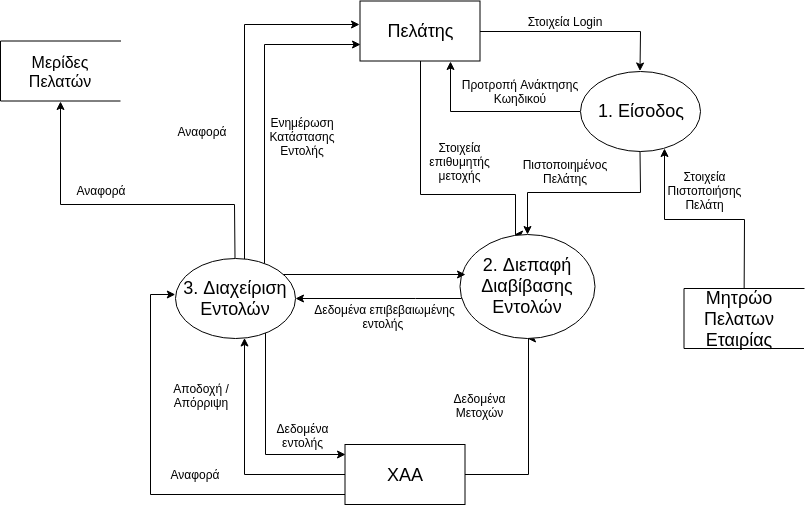
\includegraphics[width=\linewidth]{../Structured_Analysis/Level_1_Diagram.png}
	\end{figure}

	\newpage
	\subsection{Διάγραμμα Ροής Δεδομένων Επιπέδου 2}
	\subsection*{Παραδοχές}
	Η διαδικασία "2. Διεπαφή Διαβίβασης Εντολής" αναλύεται στις παρακάτω υποδιαδικασίες.
	\begin{itemize}
		\item 3.1 Επεξεργασία εντολής: 
			\begin{itemize}
				\item Ανάλυση εντολής.
				\item Πιστοποίηση πληρότητας στοιχείων χρήστη.
			\end{itemize}
		
		\item 3.2 Πληρωμή
			\begin{itemize}
				\item Διεκπεραίωση συναλλαγής με την τράπεζα.
			\end{itemize}

		\item 3.3 Επικοινωνία ΧΑΑ:
			\begin{itemize}
				\item Αποστολή εντολής στο ΧΑΑ.
				\item Συλλογή απόκρισης (Αποδοχή / Απόρριψη) από ΧΑΑ.
				\item Συλλογή αναφοράς εκκαθάρισης.
				\item Διαβίβαση πληροφορίας σε άλλες διεργασίες και σε πελάτη.
			\end{itemize}

		\item 3.4 Ενημέρωση Μερίδων:
		\begin{itemize}
			\item Υπολογισμός προμήθειας και λοιπών οικονομικών στοιχείων.
			\item Ενημέρωση μερίδας τίτλων πελάτη.
			\item Ενημέρωση ταμειακής μερίδας πελάτη.
		\end{itemize}
	\end{itemize}

	\begin{figure}[!h]
		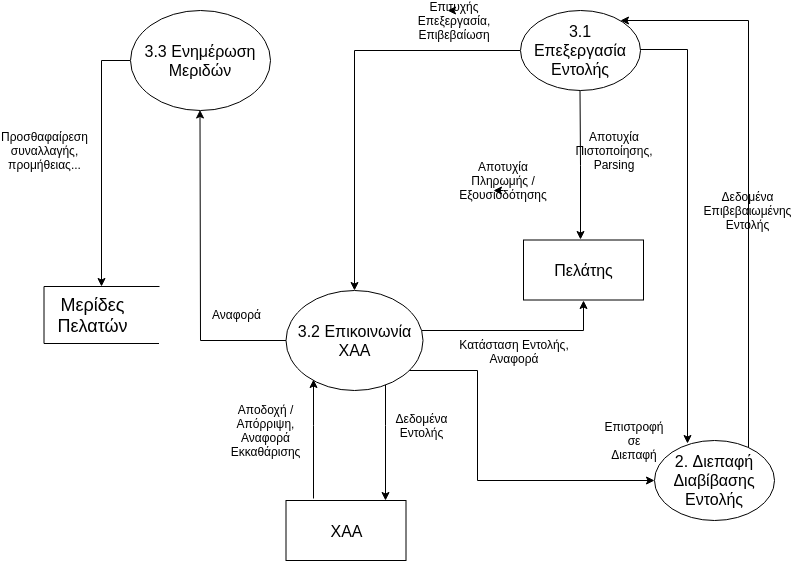
\includegraphics[width=\linewidth]{../Structured_Analysis/Level_2_Diagram.png}
	\end{figure}

\newpage
\subsection{Προδιαγραφή διαδικασίας διαβίβασης εντολής σε Δομημένα Αγγλικά}
\begin{lstlisting}
authorize_user

IF user_authorized = true
  parse_command

  IF command_is_valid = true
    authorize_payment_with_bank

    IF payment_is_valid = true
      send_command_data_to_xaa

	  IF command_is_accepted = true

	  // Asynchronous behaviour

	  await_for_xaa_execution_response
	  .then({
		IF response_is_error = true
		  send_xaa_execution_error_to_client
		ELSE
		  send_client_xaa_report
		  calculate_commission
		  update_client_portfolio
	  })

	  ELSE
	    send_xaa_error_to_client

    ELSE
      send_payment_error_to_client

  ELSE
    send_parse_error_to_client

ELSE
  send_authorization_error_to_client

redirect_to_ui

\end{lstlisting}

\newpage
\subsection{Προδιαγραφή διαδικασίας υπολογισμού προμήθειας σε Πίνακα Απόφασης}
\begin{center}
\addtolength\tabcolsep{5pt}
\begin{tabular}{ ||c|ccc|| } 
	 \hline
	 Όγκος Μετοχών & 0 - O1 & O1 - O2 & $>$ O2 \\
	 \hline
	 Προμήθεια & Π1\% & Π2\% & Π3\%\\  
	 \hline
\end{tabular}
\end{center}

\subsection{Προδιαγραφή διαδικασίας σύνδεσης του πελάτη στο σύστημα σε Δένδρο Απόφασης}
\begin{figure}[!h]
	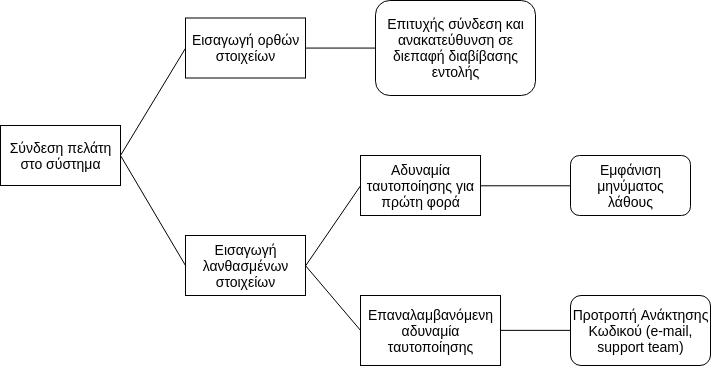
\includegraphics[width=\linewidth]{../Structured_Analysis/Decision_Tree.png}
\end{figure}

\subsection{Προδιαγραφή Λεξικού Δεδομένων αναφοράς εκκαθάρισης εντολής}
\begin{itemize}
\item Αναφορά = Αναλυτική παράθεση πράξεων αγοράς ή πώλησης + Γενικό σύνολο όγκου αγοράς + 
Συνολικό πλήθος μετοχών + Προμήθεια χρηματιστικής εταιρίας
\item Αναλυτική παράθεση πράξεων αγοράς ή πώλησης = \{Επωνυμία μετοχών + Είδος πράξης + Τιμή
 + Χρόνος + Αριθμοί τίτλων μετοχών + Πλήθος μετοχών + Συνολικό τίμημα\}
\item Είδος πράξης = [Αγορά, Πώληση]
\item Χρόνος = Ημερομηνία + Ώρα
\end{itemize}

\newpage
\subsection{Διάγραμμα αποσύνθεσης διεργασιών}

\newpage
\section{Ζητούμενα UML}
\subsection{Διάγραμμα περιπτώσεων χρήσης}
\begin{figure}[!h]
	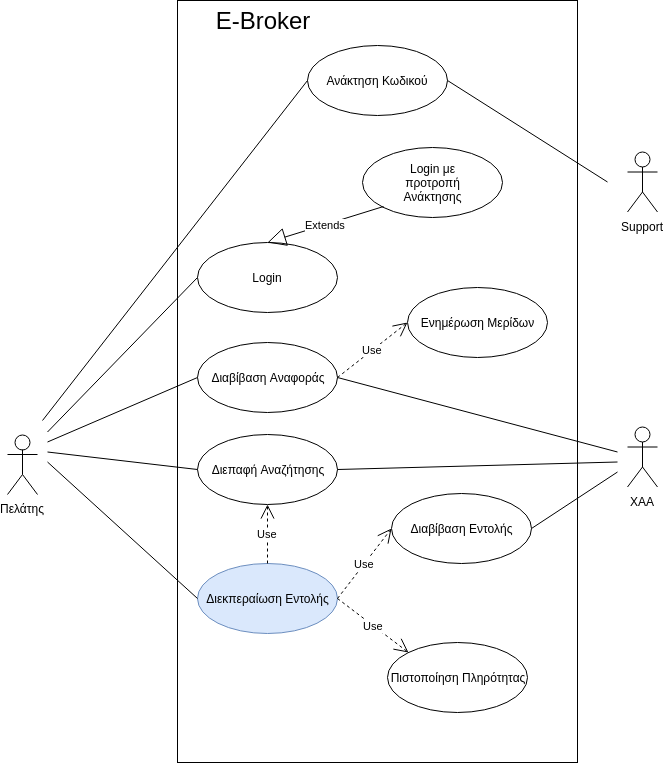
\includegraphics[width=\linewidth]{../UML/Use_Case_Diagram.png}
\end{figure}

\newpage
\subsection{Διάγραμμα κλάσσεων}
\begin{figure}[!h]
	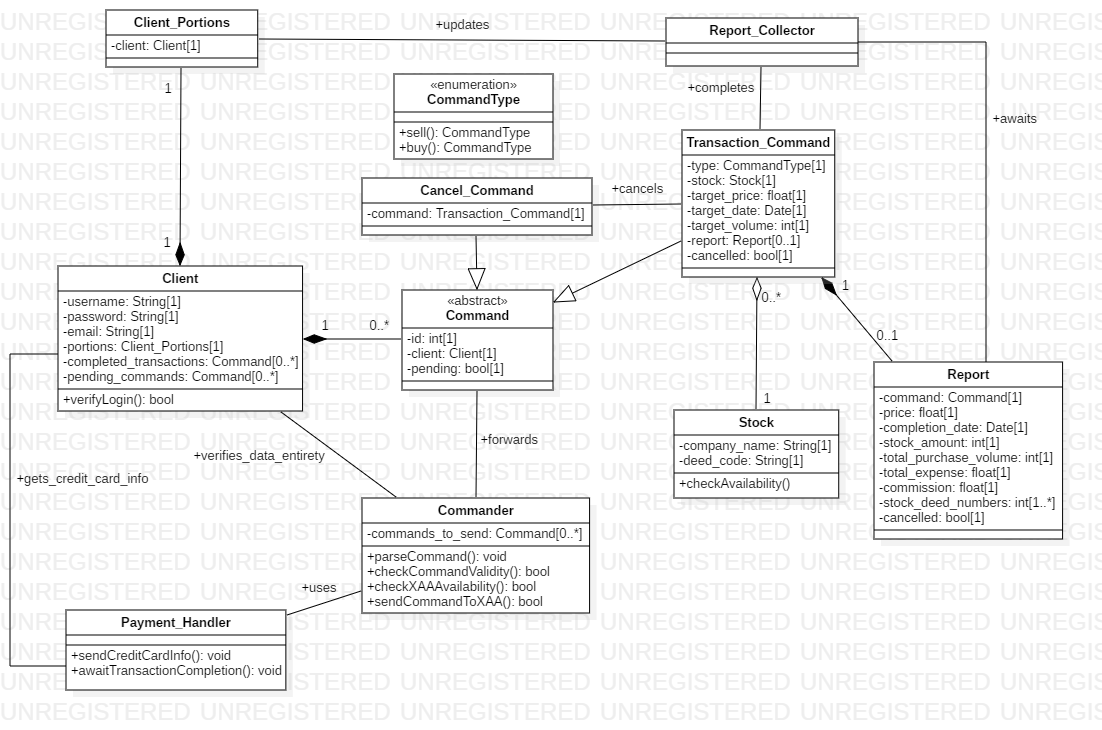
\includegraphics[width=\linewidth]{../UML/class_diagram.png}
\end{figure}

\newpage
\subsection{Διάγραμμα Καταστάσεων - Οντότητα Εντολή}
\subsection*{Παραδοχές}
Η κατάσταση "Pending" δεν θεωρείται κατάσταση δραστηριότητας, διότι όπως φαίνεται από το διάγραμμα κλάσσεων, το αντικείμενο
"Report Collector" είναι αυτό που αναμένει την αναφορά της εντολής και όχι το ίδιο το αντικείμενο "Command" (Εντολή).

\begin{figure}[!h]
	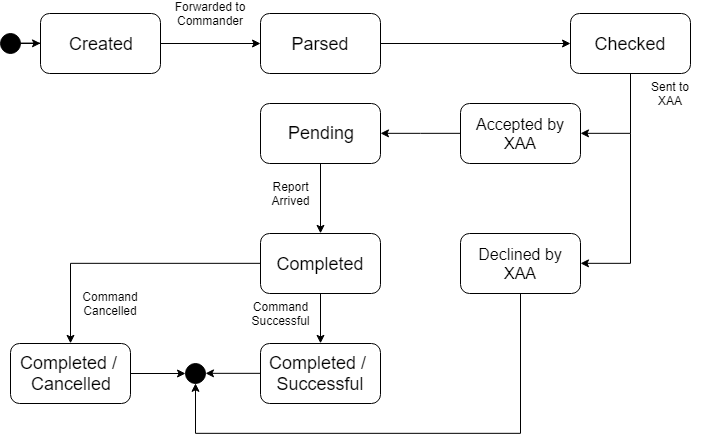
\includegraphics[width=\linewidth]{../UML/state_diagram.png}
\end{figure}

\newpage
\section{Δομημένος Σχεδιασμός}
\subsection*{Δοθέν Διάγραμμα Ροής Δεδομένων}
\begin{figure}[!h]
	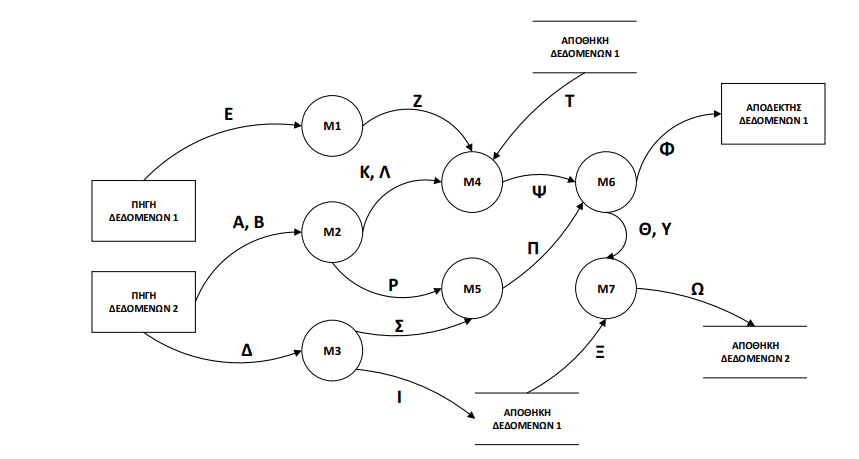
\includegraphics[width=\linewidth]{../Structured_Design/drd.png}
\end{figure}

\subsection{Διάγραμμα Δομής Προγράμματος}
\begin{figure}[!h]
	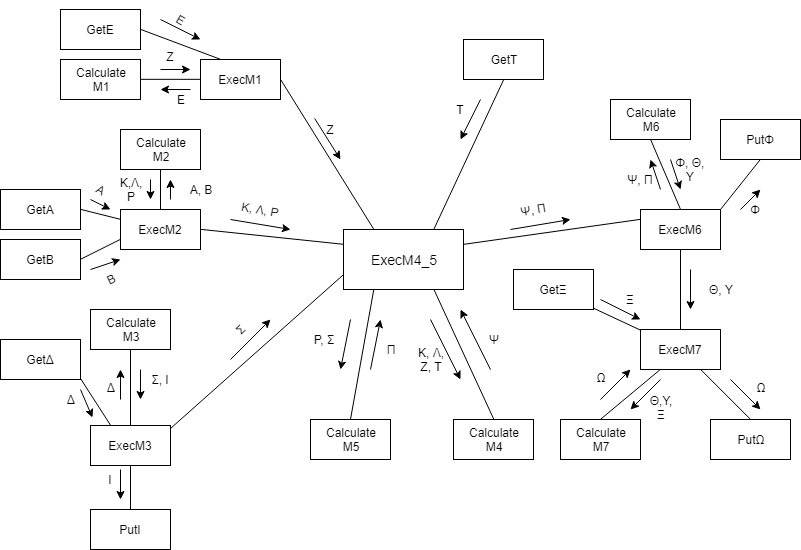
\includegraphics[width=14cm]{../Structured_Design/ddp.png}
\end{figure}

\newpage
\subsection{Ψευδοκώδικας Προγράμματος}
\subsubsection{Ψευδοκώδικας μονάδας ελέγχου Κεντρικού Μετασχηματισμού}
\begin{lstlisting}[mathescape]
Procedure ExecM4_5
  Local Var K, $\Lambda$, P, Z, T, $\Sigma$, $\Pi$, $\Psi$
  Initialize K, $\Lambda$, P, Z, T, $\Sigma$, $\Pi$, $\Psi$
  Call GetT(T)
  Call ExecM1(Z)
  Call ExecM2(K, $\Lambda$,  $\Pi$)
  Call ExecM3($\Sigma$)
  Call CalculateM4(K, $\Lambda$, P, Z, T, $\Psi$)
  Call CalculateM5(P, $\Sigma$, $\Pi$)
  Call ExecM6($\Psi$, $\Pi$)
End_Procedure
\end{lstlisting}

\subsubsection{Ψευδοκώδικας μονάδας ελέγχου Μετασχηματισμού Μ3}
\begin{lstlisting}[mathescape]
Procedure ExecM3($\Sigma$: In\Out)
  Local Var $\Delta$, $\Sigma$, I
  Initialize $\Delta$, $\Sigma$, I
  Call CalculateM3($\Delta$: In, $\Sigma$, I: In\Out)
  Call PutI(I)
End_Procedure
\end{lstlisting}

\subsubsection{Ψευδοκώδικας μονάδας υπολογισμού Μετασχηματισμού Μ4}
\begin{lstlisting}[mathescape]
Procedure CalculateM4(K, $\Lambda$, Z, T: In, $\Psi$: In\Out )
  Local Var K, $\Lambda$, Z, T, $\Psi$
  Initialize K, $\Lambda$, Z, T, $\Psi$
  Calculate $\Psi$
End_Procedure
\end{lstlisting}

\subsubsection{Ψευδοκώδικας μονάδας παρουσίασης Μετασχηματισμού Μ2}
\begin{lstlisting}[mathescape]
Procedure GetA(A: In\Out)
  Local Var A
  Initialize A
  Read A
End_Procedure

Procedure GetB(B: In\Out)
  Local Var B
  Initialize B
  Read B
End_Procedure
\end{lstlisting}

\newpage
\section{Επίλογος}


\end{document}